\newpage
\section{Results}
\label{S4}
The tool SHARPE \cite{sharpe} was used to model and derive reliability and MTTF values for the two architectures and their parts. Additionally, Gnuplot \cite{gnuplot} was used to transform the derived reliability values into graphs.

\tabref{tab:res} presents the reliability after two years of service and the MTTF (in years) for the full system and subsystems. The system bus subsystem is not presented individually, but is  incorporated in the full system. Moreover, values for both the operational modes do not need to be displayed for the CU subsystem and WU, as these modules' reliability does not change with the mode of operation.

\begin{table}[H]
\centering
 \makebox[\linewidth]{
	\begin{tabular}{| c | c | c | c |}
		\hline
		\multicolumn{2}{|c|}{Units} & Distributed & Centralized\\
		\hline
		\multirow{2}{*}{Wheel Unit} & Reliability & 0.9290 & 0.9561\\
		 & MTTF & 10.3  & 14.5\\
		\hline
		\multirow{2}{*}{Wheel Unit Subsystem Full Functionality} & Reliability & 0.7450 & 0.8357\\
		 & MTTF & 3.93  & 5.52\\
		\hline
		\multirow{2}{*}{Wheel Unit Subsystem Degraded Functionality}& Reliability & 0.9726  & 0.9891\\
		 & MTTF & 7.24 & 10.2\\
		\hline
		\multirow{2}{*}{Central Unit Subsystem}& Reliability& 0.9806  & 0.9952\\
		 & MTTF & 21.3  & 20.8\\
		\hline
		\multirow{2}{*}{Full System Full Functionality}& Reliability & 0.7305  & 0.8316\\
		 & MTTF & 3.74 & 5.23\\
		\hline
		\multirow{2}{*}{Full System Degraded Functionality}& Reliability & 0.9537 & 0.9843\\
		 & MTTF & 6.56 & 9.06\\
		\hline
	\end{tabular}
}
\caption{The table presents the reliability after four years of service and the MTTF (years) for several units.}
\label{tab:res}
\end{table}
\figref{fig:wu} presents the reliability graph for a single WU, \figref{fig:wus} presents the reliability graph for the WU subsystem, \figref{fig:cu} presents the reliability graph for the CU subsystem, and \figref{fig:fs} presents the reliability graph for the full system. All reliability graphs display curves for both the full functionality mode and the degraded (deg) mode, as well as for both the centralized (cent) and the distributed (dist) design. However, the reliability graphs for a WU and the CU subsystem only has two curves, which is due to that they have the same reliability in both operating modes. 

\begin{figure}[H]
  \centering
  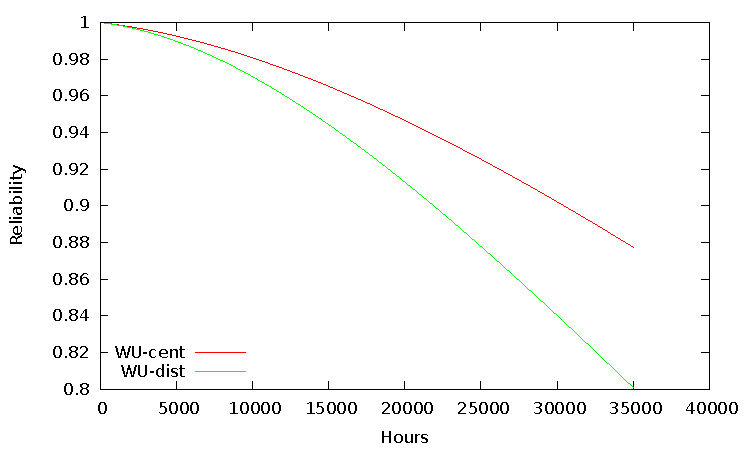
\includegraphics{plots/WU.pdf}
  \caption{Reliability graph for a WU for both architectures.}
  \label{fig:wu}
\end{figure}

\begin{figure}[H]
  \centering
  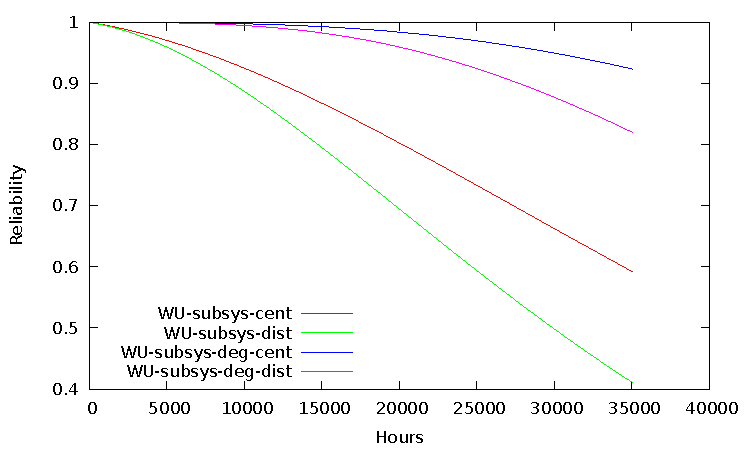
\includegraphics{plots/WUs.pdf}
  \caption{Reliability graph for a WU subsystem in the two failure modes for both architectures.}
  \label{fig:wus}
\end{figure}

\begin{figure}[H]
  \centering
  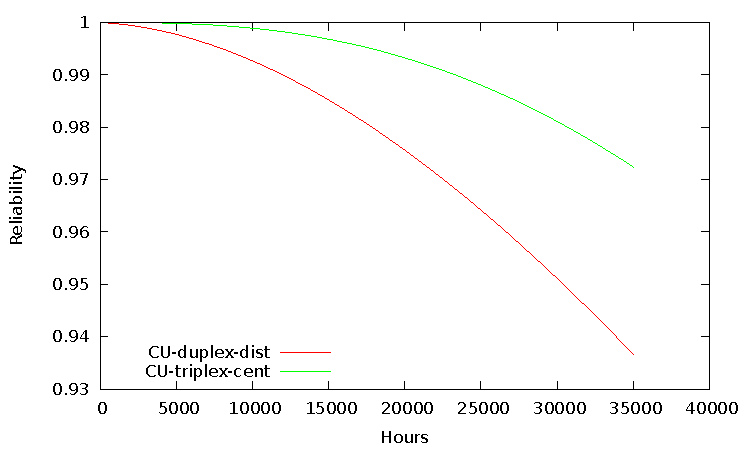
\includegraphics{plots/CUs.pdf}
  \caption{Reliability graph for a CU subsystem in the two failure modes for both architectures.}
  \label{fig:cu}
\end{figure}

\begin{figure}[H]
  \centering
  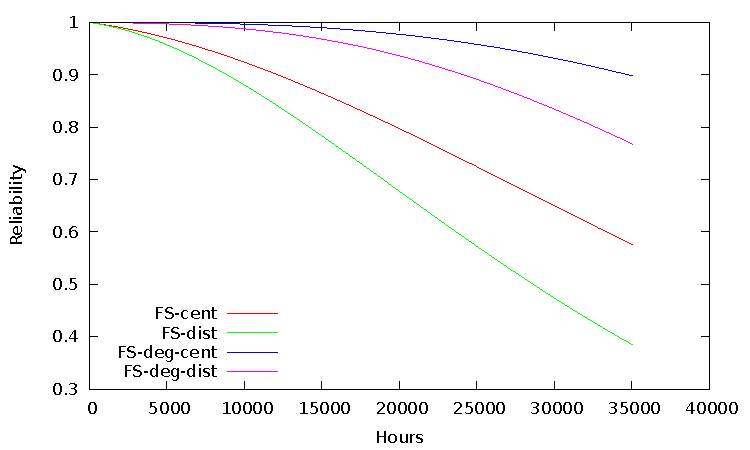
\includegraphics{plots/FS.pdf}
  \caption{Reliability graph for the full system in the two failure modes for both architectures.}
  \label{fig:fs}
\end{figure}

The hours of service before 0.92 reliability was reached for the full systems in degraded mode is presented in \figref{fig:cfs_hf}. The centralized design operate 45\% longer than the distributed design, 31860  h versus 21960 h, respectively. If the failure rate of the computer modules in the CU for the centralized architecture was increased to $22.21 \time 10^{-6}$, the time of service coincide with the distributed design at 0.92 reliability, as shown by the `highfail' curve in \figref{fig:cfs_hf}. 
\begin{figure}[H]
  \centering
  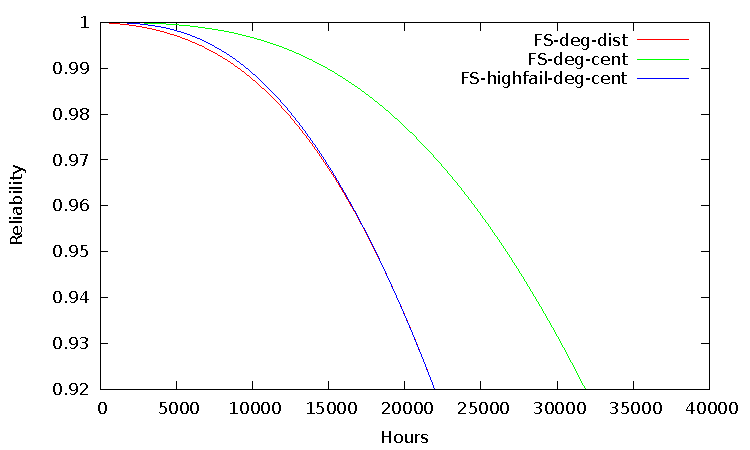
\includegraphics{plots/3b.pdf}
  \caption{Reliability graph for the full system in degraded mode for both architectures, as well as for the full system in degradede mode for the centralized design when the failure rate of the computing modules in the CU is increased.}
  \label{fig:cfs_hf}
\end{figure}